\begin{frame}
    \frametitle{\problemtitle}

    \begin{columns}
        \begin{column}[T]{.70\textwidth}
            \begin{itemize}
                \item Calculate the minimum radius of a stroopwafel with strictly more than $1 \leq s \leq 10^9$ squares.
                \item The area of each square is $1~\text{cm}^2$.
                \item The centre point of the stroopwafel always contains the common
                corner of the four adjacent squares in the centre
                (i.e., the squares are aligned to a Cartesian grid).
            \end{itemize}

            \vspace{1em}

            \centering
            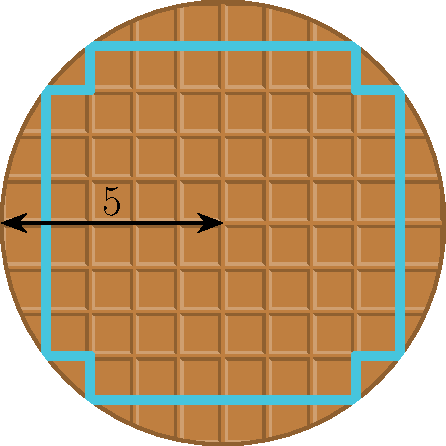
\includegraphics[width=0.25\textwidth]{sample}

            \small
            Illustration of Sample Input 2, with the blue-enclosed region depicting
            the $60$ whole squares that the cookie contains.
            The required radius is exactly $5.0~\text{cm}$.
        \end{column}

        \illustration{.25}{cookie}{A traditional circular caramel cookie (stroopwafel).}% Source: Own work
    \end{columns}
\end{frame}
